\section*{Segmentation}

Goal: partition the pixels of an image into \textbf{groups} that
strongly correlate with the \textbf{objects} in an image

Typically the \textbf{first step} in any automated computer vision application

\subsection*{Detection of Discontinuities}

\subsubsection*{Point Detection}

The following filter is applied, then the pixels above a certain
threshold are considered points:

\vspace{-0.3cm}
\begin{figure}[H]
  \centering
  \begin{tikzpicture}[%
      filtercell/.style={draw=MaterialBlue900, fill=MaterialBlue50,
      minimum size=1cm, anchor=center}
    ]
    \node[filtercell] (f11) at (0,2) {$-1$};
    \node[filtercell] (f12) at (1,2) {$-1$};
    \node[filtercell] (f13) at (2,2) {$-1$};
    \node[filtercell] (f21) at (0,1) {$-1$};
    \node[filtercell] (f22) at (1,1) {$8$};
    \node[filtercell] (f23) at (2,1) {$-1$};
    \node[filtercell] (f31) at (0,0) {$-1$};
    \node[filtercell] (f32) at (1,0) {$-1$};
    \node[filtercell] (f33) at (2,0) {$-1$};

  \end{tikzpicture}
  \caption{Point detection filter}
\end{figure}

\subsubsection*{Line Detection}

Masks below extract one pixel thick lines running in a particular direction:

\begin{figure}[ht]
  \centering
  % first row
  \begin{subfigure}[t]{0.5\linewidth}
    \centering
    % Horizontal filter
    \begin{tikzpicture}[filtercell/.style={
          draw=MaterialBlue900, fill=MaterialBlue50,
      minimum size=1cm, inner sep=0pt, outer sep=0pt}]
      \foreach \x in {0,1,2}{
        \node[filtercell] at (\x,2) {$-1$};
        \node[filtercell] at (\x,1) {$ 2$};
        \node[filtercell] at (\x,0) {$-1$};
      }
    \end{tikzpicture}
    \subcaption{Horizontal}
  \end{subfigure}%
  \begin{subfigure}[t]{0.48\linewidth}
    \centering
    % Vertical filter
    \begin{tikzpicture}[filtercell/.style={
          draw=MaterialBlue900, fill=MaterialBlue50,
      minimum size=1cm, inner sep=0pt, outer sep=0pt}]
      \foreach \y in {0,1,2}{
        \node[filtercell] at (0,\y) {$-1$};
        \node[filtercell] at (1,\y) {$ 2$};
        \node[filtercell] at (2,\y) {$-1$};
      }
    \end{tikzpicture}
    \subcaption{Vertical}
  \end{subfigure}

  \bigskip  % vertical gap

  % second row
  \begin{subfigure}[t]{0.48\linewidth}
    \centering
    % Diagonal (\) filter
    \begin{tikzpicture}[filtercell/.style={
          draw=MaterialBlue900, fill=MaterialBlue50,
      minimum size=1cm, inner sep=0pt, outer sep=0pt}]
      \node[filtercell] at (0,2) {$-1$};
      \node[filtercell] at (1,2) {$-1$};
      \node[filtercell] at (2,2) {$ 2$};
      \node[filtercell] at (0,1) {$-1$};
      \node[filtercell] at (1,1) {$ 2$};
      \node[filtercell] at (2,1) {$-1$};
      \node[filtercell] at (0,0) {$ 2$};
      \node[filtercell] at (1,0) {$-1$};
      \node[filtercell] at (2,0) {$-1$};
    \end{tikzpicture}
    \subcaption{Diagonal ($+45^\circ$)}
  \end{subfigure}%
  \begin{subfigure}[t]{0.48\linewidth}
    \centering
    % Diagonal (/) filter
    \begin{tikzpicture}[filtercell/.style={
          draw=MaterialBlue900, fill=MaterialBlue50,
      minimum size=1cm, inner sep=0pt, outer sep=0pt}]
      \node[filtercell] at (0,2) {$ 2$};
      \node[filtercell] at (1,2) {$-1$};
      \node[filtercell] at (2,2) {$-1$};
      \node[filtercell] at (0,1) {$-1$};
      \node[filtercell] at (1,1) {$ 2$};
      \node[filtercell] at (2,1) {$-1$};
      \node[filtercell] at (0,0) {$-1$};
      \node[filtercell] at (1,0) {$-1$};
      \node[filtercell] at (2,0) {$ 2$};
    \end{tikzpicture}
    \subcaption{Diagonal ($-45^\circ$)}
  \end{subfigure}

  \caption{Line‐detection filters in four orientations.}
\end{figure}

\subsubsection*{Edge Detection}

An \textbf{edge} is a set of connected pixels that lie on the
boundary between two regions.

\begin{figure}[H]
  \centering
  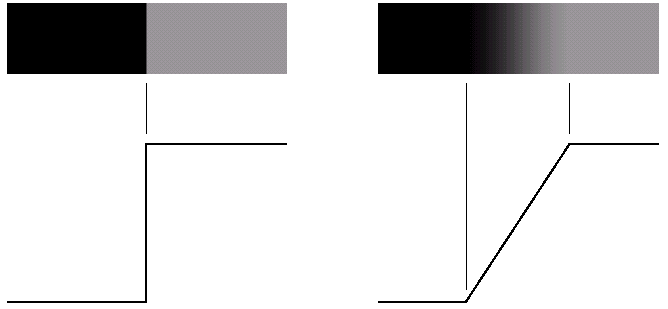
\includegraphics[width=\linewidth]{images/edge_models.png}
  \caption{Two common edge models: ideal (step) and ramp}
\end{figure}

Note: Derivative-based edge detectors are \textbf{extremely sensitive to noise}.

\textbf{Common edge detectors}:

\begin{itemize}

  \item \textbf{Roberts}

    \begin{minipage}{\linewidth}
      \vspace{-0.3cm}
      \begin{figure}[H]
        \centering
        \begin{tikzpicture}[%
            filtercell/.style={draw=MaterialBlue900, fill=MaterialBlue50,
            minimum size=1cm, anchor=center}
          ]
          % G_x
          \node[filtercell] (r111) at (0,1) {$-1$};
          \node[filtercell] (r112) at (1,1) {$0$};
          \node[filtercell] (r121) at (0,0) {$0$};
          \node[filtercell] (r122) at (1,0) {$1$};
          % G_y
          \node[filtercell] (r211) at (3,1) {$0$};
          \node[filtercell] (r212) at (4,1) {$-1$};
          \node[filtercell] (r221) at (3,0) {$1$};
          \node[filtercell] (r222) at (4,0) {$0$};
        \end{tikzpicture}
        \caption{Roberts filters for $G_x$ (left) and $G_y$ (right)}
      \end{figure}
    \end{minipage}

  \item \textbf{Prewitt}

    \begin{minipage}{\linewidth}
      \vspace{-0.3cm}
      \begin{figure}[H]
        \centering
        \begin{tikzpicture}[%
            filtercell/.style={draw=MaterialBlue900, fill=MaterialBlue50,
            minimum size=1cm, anchor=center}
          ]
          % G_x
      
          \node[filtercell] (p111) at (0,2) {$-1$};
          \node[filtercell] (p112) at (1,2) {$0$};
          \node[filtercell] (p113) at (2,2) {$1$};
          \node[filtercell] (p121) at (0,1) {$-1$};
          \node[filtercell] (p122) at (1,1) {$0$};
          \node[filtercell] (p123) at (2,1) {$1$};
          \node[filtercell] (p131) at (0,0) {$-1$};
          \node[filtercell] (p132) at (1,0) {$0$};
          \node[filtercell] (p133) at (2,0) {$1$};
          % G_y
          \node[filtercell] (p211) at (4,2) {$-1$};
          \node[filtercell] (p212) at (5,2) {$-1$};
          \node[filtercell] (p213) at (6,2) {$-1$};
          \node[filtercell] (p221) at (4,1) {$0$};
          \node[filtercell] (p222) at (5,1) {$0$};
          \node[filtercell] (p223) at (6,1) {$0$};
          \node[filtercell] (p231) at (4,0) {$1$};
          \node[filtercell] (p232) at (5,0) {$1$};
          \node[filtercell] (p233) at (6,0) {$1$};
          
        \end{tikzpicture}
        \caption{Prewitt filters for $G_x$ (left) and $G_y$ (right)}
      \end{figure}
    \end{minipage}

  \item \textbf{Sobel}

    \begin{minipage}{\linewidth}
      \vspace{-0.3cm}
      \begin{figure}[H]
        \centering
        \begin{tikzpicture}[%
            filtercell/.style={draw=MaterialBlue900, fill=MaterialBlue50,
            minimum size=1cm, anchor=center}
          ]
          % G_x
          \node[filtercell] (s111) at (0,2) {$-1$};
          \node[filtercell] (s112) at (1,2) {$0$};
          \node[filtercell] (s113) at (2,2) {$1$};
          \node[filtercell] (s121) at (0,1) {$-2$};
          \node[filtercell] (s122) at (1,1) {$0$};
          \node[filtercell] (s123) at (2,1) {$2$};
          \node[filtercell] (s131) at (0,0) {$-1$};
          \node[filtercell] (s132) at (1,0) {$0$};
          \node[filtercell] (s133) at (2,0) {$1$};
          % G_y
          \node[filtercell] (s211) at (4,2) {$-1$};
          \node[filtercell] (s212) at (5,2) {$-2$};
          \node[filtercell] (s213) at (6,2) {$-1$};
          \node[filtercell] (s221) at (4,1) {$0$};
          \node[filtercell] (s222) at (5,1) {$0$};
          \node[filtercell] (s223) at (6,1) {$0$};
          \node[filtercell] (s231) at (4,0) {$1$};
          \node[filtercell] (s232) at (5,0) {$2$};
          \node[filtercell] (s233) at (6,0) {$1$};
        \end{tikzpicture}
        \caption{Sobel filters for $G_x$ (left) and $G_y$ (right)}
      \end{figure}
    \end{minipage}

  \item \textbf{Laplacian of Gaussian:} The \textbf{Laplacian} is
    typically not used by itself as it is very sensitive to noise; so
    we combine it with a smoothing operator (Gaussian). This is also
    known as the \textbf{Mexican hat} filter.

    \begin{minipage}{\linewidth}
      \vspace{-0.3cm}
      \begin{figure}[H]
        \centering
        \begin{tikzpicture}[%
            filtercell/.style={draw=MaterialBlue900, fill=MaterialBlue50,
            minimum size=1cm, anchor=center}
          ]
          % Row y=4
          \node[filtercell] at (0,4) {$0$};
          \node[filtercell] at (1,4) {$0$};
          \node[filtercell] at (2,4) {$-1$};
          \node[filtercell] at (3,4) {$0$};
          \node[filtercell] at (4,4) {$0$};
          % Row y=3
          \node[filtercell] at (0,3) {$0$};
          \node[filtercell] at (1,3) {$-1$};
          \node[filtercell] at (2,3) {$-2$};
          \node[filtercell] at (3,3) {$-1$};
          \node[filtercell] at (4,3) {$0$};
          % Row y=2
          \node[filtercell] at (0,2) {$-1$};
          \node[filtercell] at (1,2) {$-2$};
          \node[filtercell] at (2,2) {$16$};
          \node[filtercell] at (3,2) {$-2$};
          \node[filtercell] at (4,2) {$-1$};
          % Row y=1
          \node[filtercell] at (0,1) {$0$};
          \node[filtercell] at (1,1) {$-1$};
          \node[filtercell] at (2,1) {$-2$};
          \node[filtercell] at (3,1) {$-1$};
          \node[filtercell] at (4,1) {$0$};
          % Row y=0
          \node[filtercell] at (0,0) {$0$};
          \node[filtercell] at (1,0) {$0$};
          \node[filtercell] at (2,0) {$-1$};
          \node[filtercell] at (3,0) {$0$};
          \node[filtercell] at (4,0) {$0$};
        \end{tikzpicture}
        \caption{Laplacian‐of‐Gaussian (LoG) filter}
      \end{figure}
    \end{minipage}

    \begin{minipage}{\linewidth}
      \begin{figure}[H]
        \centering
        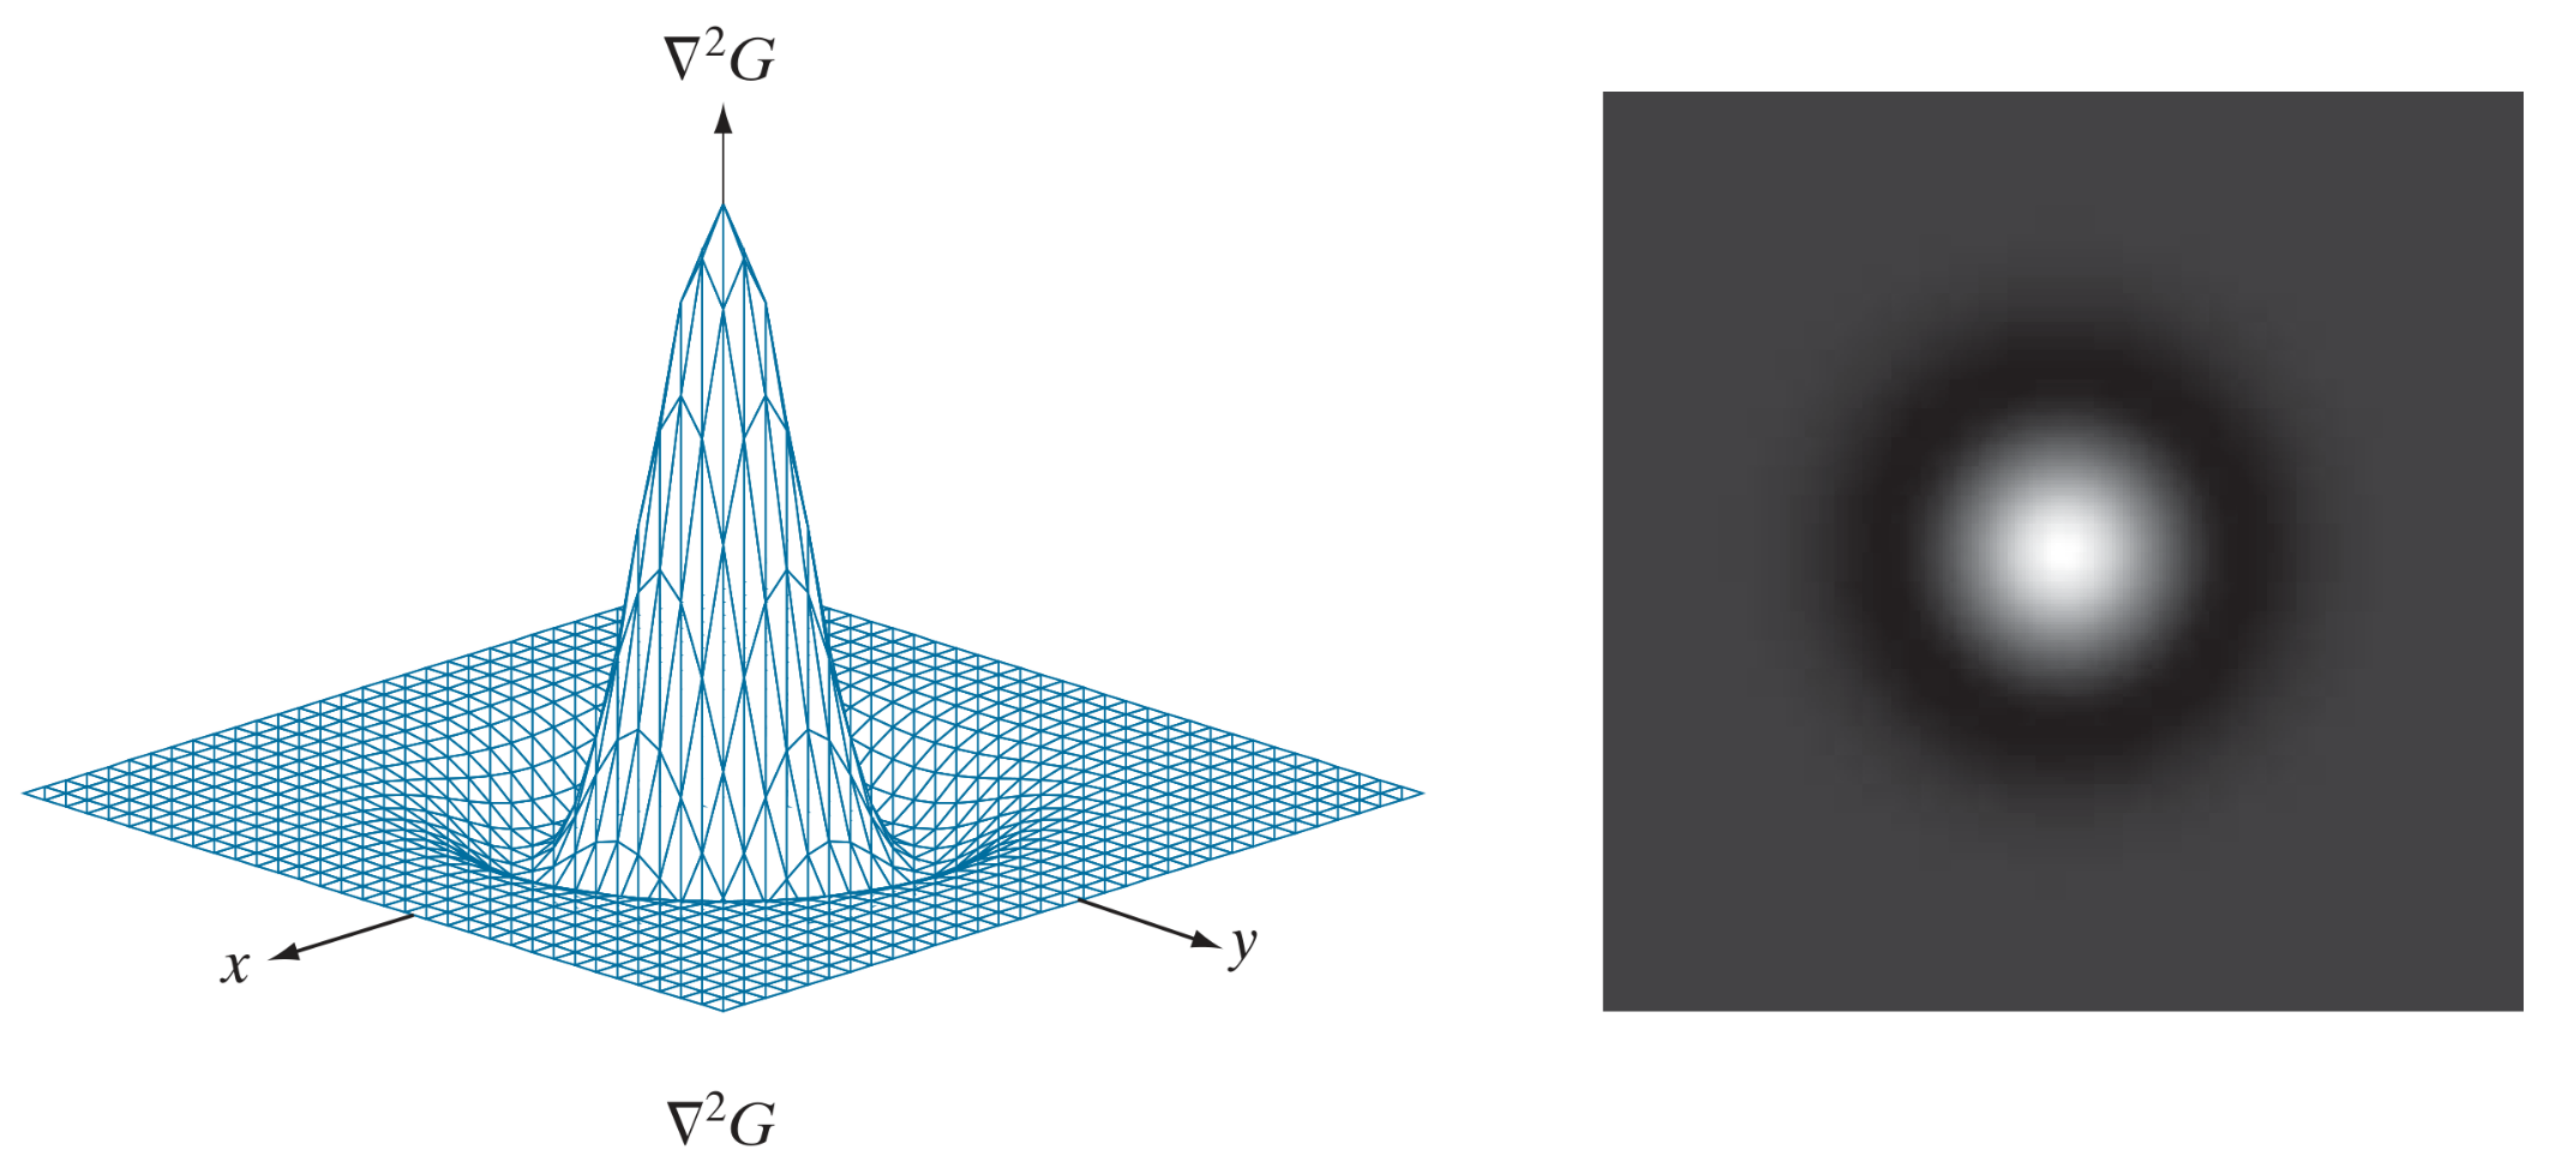
\includegraphics[width=\linewidth]{images/laplacian_of_gaussian.png}
        \caption{Plot of the Mexican hat filter}
      \end{figure}
    \end{minipage}
\end{itemize}
